
%%%%%%%%%%%%%%%%%%%%%%% file typeinst.tex %%%%%%%%%%%%%%%%%%%%%%%%%
%
% This is the LaTeX source for the instructions to authors using
% the LaTeX document class 'llncs.cls' for contributions to
% the Lecture Notes in Computer Sciences series.
% http://www.springer.com/lncs       Springer Heidelberg 2006/05/04
%
% It may be used as a template for your own input - copy it
% to a new file with a new name and use it as the basis
% for your article.
%
% NB: the document class 'llncs' has its own and detailed documentation, see
% ftp://ftp.springer.de/data/pubftp/pub/tex/latex/llncs/latex2e/llncsdoc.pdf
%
%%%%%%%%%%%%%%%%%%%%%%%%%%%%%%%%%%%%%%%%%%%%%%%%%%%%%%%%%%%%%%%%%%%


\documentclass[runningheads,a4paper]{llncs}


\setcounter{tocdepth}{3}
\usepackage{graphicx}
%
\usepackage{mathptmx}      % use Times fonts if available on your TeX system
%
% insert here the call for the packages your document requires
\usepackage{latexsym}
\usepackage{url}
\usepackage{changepage}
\usepackage{amssymb,amsmath}
\usepackage[colorlinks,citecolor=blue,linkcolor=blue]{hyperref}
\usepackage{color}
\usepackage{mdwlist}
\usepackage{algorithm}
\usepackage{algorithmic}
\renewcommand{\algorithmicrequire}{ \textbf{Input:}} %Use Input in the format of Algorithm
\renewcommand{\algorithmicensure}{ \textbf{Output:}} %UseOutput in the format of Algorithm
%\spnewtheorem{definition}{Definition}{\bf}{\rm}
\spnewtheorem{hypothesis}{Hypothesis}{\bf}{\rm}

\usepackage{url}
\urldef{\mailsa}\path|{alfred.hofmann, ursula.barth, ingrid.haas, frank.holzwarth,|
\urldef{\mailsb}\path|anna.kramer, leonie.kunz, christine.reiss, nicole.sator,|
\urldef{\mailsc}\path|erika.siebert-cole, peter.strasser, lncs}@springer.com|    
\newcommand{\keywords}[1]{\par\addvspace\baselineskip
\noindent\keywordname\enspace\ignorespaces#1}

\begin{document}

\mainmatter  % start of an individual contribution

% first the title is needed
\title{Mining Topics Related Opinions of Users on Social Media: Generative Way or Not?}

% a short form should be given in case it is too long for the running head
\titlerunning{Lecture Notes in Computer Science: Authors' Instructions}

% the name(s) of the author(s) follow(s) next
%
% NB: Chinese authors should write their first names(s) in front of
% their surnames. This ensures that the names appear correctly in
% the running heads and the author index.
%
\author{Alfred Hofmann%
\thanks{Please note that the LNCS Editorial assumes that all authors have used
the western naming convention, with given names preceding surnames. This determines
the structure of the names in the running heads and the author index.}%
\and Ursula Barth\and Ingrid Haas\and Frank Holzwarth\and\\
Anna Kramer\and Leonie Kunz\and Christine Rei\ss\and\\
Nicole Sator\and Erika Siebert-Cole\and Peter Stra\ss er}
%
\authorrunning{Lecture Notes in Computer Science: Authors' Instructions}
% (feature abused for this document to repeat the title also on left hand pages)

% the affiliations are given next; don't give your e-mail address
% unless you accept that it will be published
\institute{Springer-Verlag, Computer Science Editorial,\\
Tiergartenstr. 17, 69121 Heidelberg, Germany\\
\mailsa\\
\mailsb\\
\mailsc\\
\url{http://www.springer.com/lncs}}

%
% NB: a more complex sample for affiliations and the mapping to the
% corresponding authors can be found in the file "llncs.dem"
% (search for the string "\mainmatter" where a contribution starts).
% "llncs.dem" accompanies the document class "llncs.cls".
%

\toctitle{Lecture Notes in Computer Science}
\tocauthor{Authors' Instructions}
\maketitle


\begin{abstract}
Social media such as Twitter, has enabled more and more people to freely express their opinions on the web, making it an extremely valuable source for mining opinions of users about all kinds of topics. In this paper we study how to automatically integrate opinions expressed by a user in not so well-written User-Generated Content (UGC). Several generative topic-sentiment mixture models (TSM) have been designed to capture sentiments and topics in text simultaneously. We propose a subjectivity model by combining topics a user talks about and his opinions towards these topics. In constrast to TSM model, we estimate our model with LDA topic model and sentiment analysis techniques in a separate way based on user-level data. We compare our model and TSM model in a series of experiments on Twitter data. Experiments on integrating opinions show that the proposed method is effective and can generate useful aligned integrated opinion summaries of users. Futhermore, the proposed method can catch more fine-grain opinions than TSM model and get better performance in a friend recommendation task. 
\keywords{TSM model, Twitter, sentiment analysis, Twitter, LDA}
\end{abstract}

\section{Introduction}

With the dramatic rise of text-based social media such as Twitter, millions of users are more and more willing to publish online short messages to express their opinions on a great variety of topics. The wide coverage of topics, dynamics of discussion, and abundance of opinions imbeded in the social media data make them extremely valuable for mining user opinions about all kinds of topics (e.g., products, political figures, etc.), which in turn can enable a wide range of applications, such as opinion search for ordinary users, opinion tracking for business intelligence, and user behavior prediction for targeted advertising. 
However, with such a large scale of information source, it is quite challenging for a user to integrate and digest all the opinions from different users. For example, a query ``iPhone'' returns 830,879 matches of 231,233 users on Twitter (as of Jan. 14, 2014), suggesting that there are many users have expressed opinions more than once about iPhone on Twitter. To enable a user to benefit from all kinds of opinions of different users, it is thus necessary to automatically integrate and present an integrated opinion summary for each user \cite{lu2008opinion}. In fact, users often publish many messages on the topics they are interested in, therefore how to find these topics and integrate opinions towards each topic poses special challenge for opinion mining related researchers.

In this paper, we propose a two-parts model by incorporating topic modeling and sentiment analysis into one framework in a separated way illustrated as in Figure~\ref{fig1}, in which part 1 represents topics of interest distribution of users, while part 2 represents the distribution of opinions towards these topics. Specifically, we propose a general method to solve this integration problem in three steps: (1) extract topics of interest from tweets of a user using user-level LDA; (2) extract separated sentiment and topic for each tweet with sentiment and topic analysis  (3) summarize and integrate the extracted opinions towards topics.
\begin{figure}[htb]
\centering
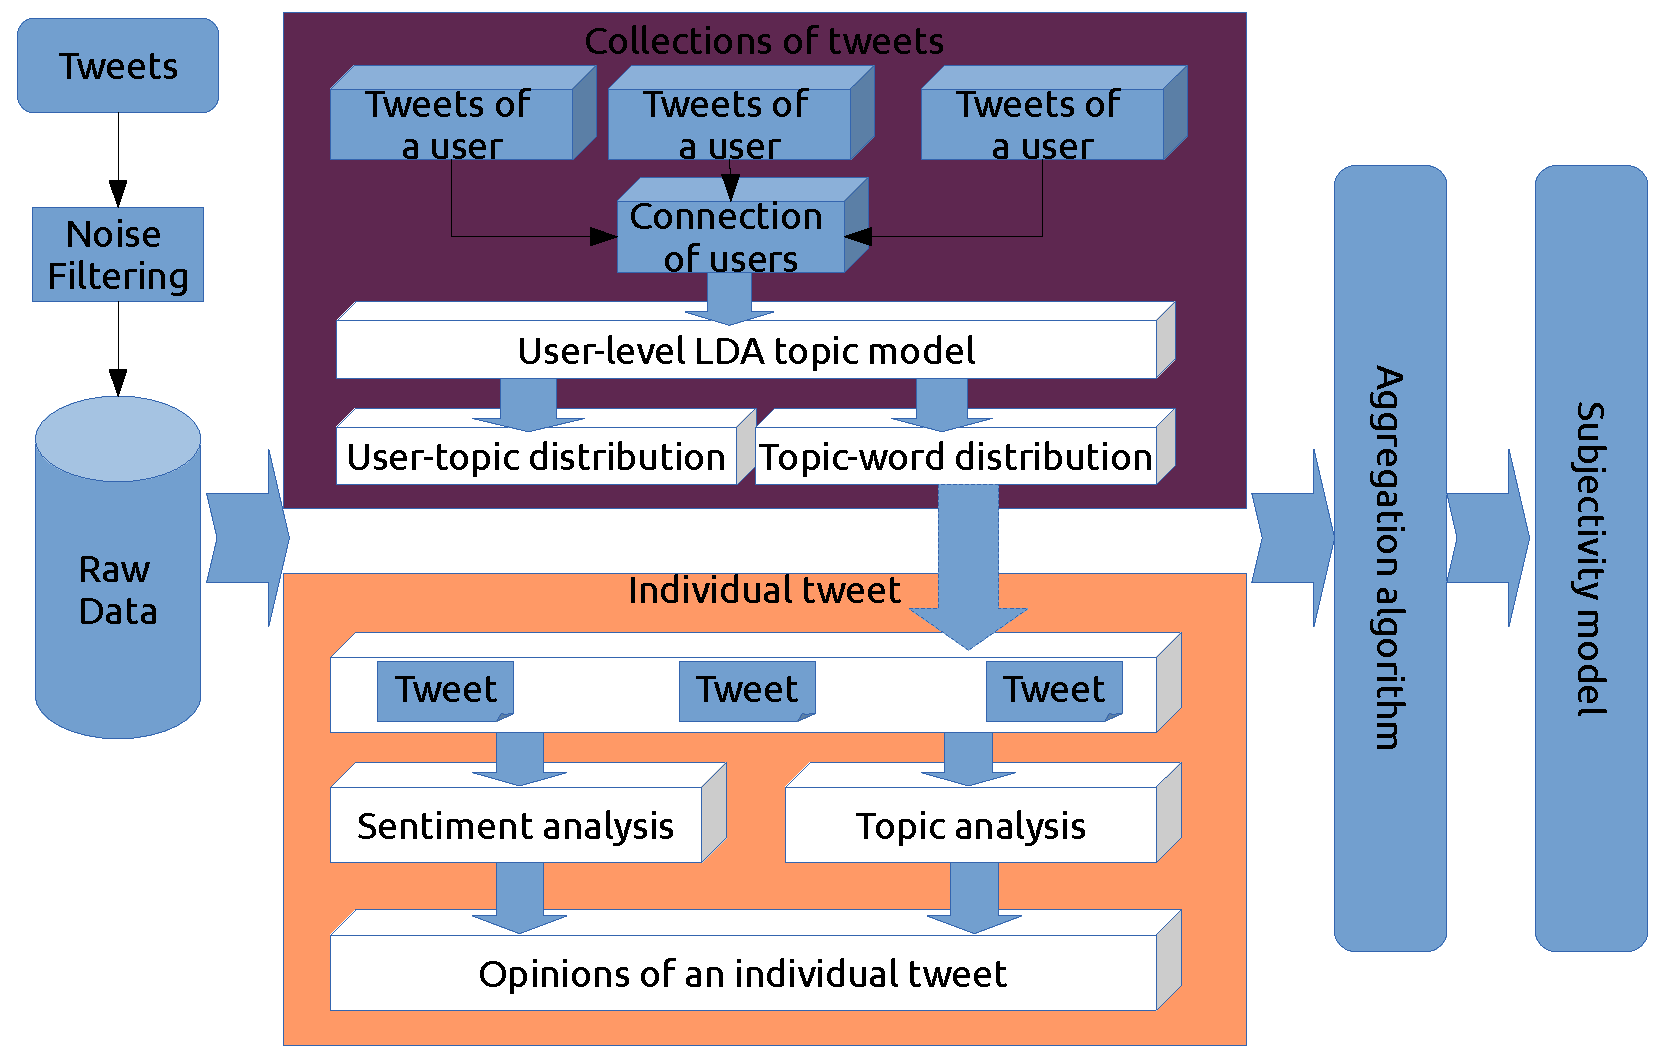
\includegraphics[width=5.0in,height=3.0in]{procedure.pdf}
\caption{Framework of two-parts subjectivity model.}
\label{fig1}
\end{figure}


Several studies have tried to meet such a challenge by integrating sentiment into a generative topic model. Mei \emph{et al.}~\cite{mei2007topic} proposed Topic-Sentiment Mixture (TSM) model that can reveal latent topics of a blog, and the topics associated sentiments. Lin \emph{et al.}~\cite{lin2009joint} proposed a Joint Sentiment/Topic (JST) model based on LDA that can detect topic and sentiment simultaneously. Both TSM and JST tried to model topic and sentiment at the same time in a generative way. Specifically they learn a general word-sentiment distribution to model the sentiment of blogs or reviews, which may not work well for short and informal social media languages such as tweets. Sentiment of tweets is determined not only by formal words but also by various special characteristics of Twitter languages such as emoticon, capitalized words, repeated letters and exclamation mark, etc. Those features can not be easily modeled by a probabilistic distribution.  However, rule-based sentiment analysis methods can catch some subtle sentiment of tweets by transforming these characteristics into rules. 


We propose to improve sentiment analysis by utilizing the information about user-user relationships made evident by online social networks. We do so for two reasons. First, user-relationship information is now more easily obtainable, since user-generated content often appears in the context of social media. For example, Twitter maintains not just tweets, but also lists of followers and followees. Second, and more importantly, when a user forms a link in a network such as Twitter, they do so to create a connection. If this connection corresponds to a personal relationship, then the principle of homophily \cite{lazarsfeld_friendship_1954} — the idea that similarity and connection tend to cooccur, or ``birds of a feather flock together'' \cite{mcpherson2001birds} —suggests that users that are``connected'' by a mutual personal relationship may tend to hold similar opinions; indeed, one study found some evidence of homophily for both positive and negative sentiment among MySpace Friends \cite{thelwall2010emotion}. Alternatively, the connection a user creates may correspond to approval (e.g., of a famous figure) or a desire to pay attention (e.g., to a news source), rather than necessarily a personal relationship; but such connections are still also suggestive of the possibility of a shared opinion.
we incorporate user-relation information, as follows. We first utilize a model based on the follower/followee network that has dependencies not only between the opinion of a user and the opinions expressed in his/her tweets, but also be- tween his/her opinion and those of the users that he/she follows.
We work within a semi-supervised, user-level framework.We focus on user-level rather than tweet-level (corresponding to document- or sentence-level) sentiment because the end goal for many users of opinion-mining technologies is to find out what peo- ple think; determining the sentiment expressed in individual texts is usually a subtask of or proxy for that ultimate objective. Addition- ally, it is plausible that there are cases where some of a user’s tweets are genuinely ambiguous (perhaps because they are very short), but his/her overall opinion can be determined by looking at his/her col- lection of tweets and who he/she is connected to.\cite{tan2011user}
we frame the problem in the context of Twitter to keep things concrete, although adaptation of this framework to other social-network settings is straightforward. In brief, we ad- dress the semi-supervised topic-dependent sentiment-polarity user categorization task.
Our task is to classify each user’s sentiment on a specific topic
into one of two polarities: “Positive” and “Negative”.(We initially worked with positive/negative/neutral labels, but de- termining neutrality was difficult for the annotators). “Positive” means that the user supports or likes the target topic, whereas “Neg- ative” stands for the opposite. (As stated above, this differs from classifying each of a user’s tweets.)
This corresponds to the idea that users often agree with those they pay attention to.
In this section, we give a formal definition of the model we work
with. 
The main advantage of our formulation is that it employs social-network structure to help us overcome both the paucity of textual information in short tweets and the lack of a large amount of labeled data.

This paper presents a comparative study of three closely related Bayesian mod- els for unsupervised document level senti- ment classification, namely, the latent sen- timent model (LSM), the joint sentiment- topic (JST) model, and the Reverse-JST model.\cite{lin2010comparative}

We show a typical scenario of topic level opinion influence analysis on TencentMicroblog (a chinese microblogging website) in Figure 1


We now address the problems of estimating the remaining free parameters and inferring user sentiment labels once the parameter values have been learned.

There’re two important factors that should be taken into consider- ations. One, opinions and topics are closely related. The online discussions around some entity, or object, often cover a mixture of features/topics related to that entity with different preferentials. Different opinions may be expressed by users towards different topics, where users may like some aspects of an entity but dislike other aspects. Two, users’ opinions are subject to social influence. The rise of social media puts the sentiment analysis in the context of social network. Users not only express their individual opinions, but also exchange opinions with others. In the context of opinion mining, social influence refers to the phenomenon that one is inclined to agree (positive influence) or disagree (negative influence) with his/her neighbors’ opinions with different degrees, depending on the influence strengths.


This paper makes the following contributions:
1.We define a new problem of opinion integration. To the best of our knowledge, there is no existing work that solves this problem.
2. We propose a new semi-supervised topic modeling ap- proach for integrating opinions scattered around in text articles with those in a well-written expert review for an arbitrary topic.
3. We evaluate the proposed method both qualitatively and quantitatively. The results show that our method is effective for integrating opinions about quite differ- ent topics.
Collecting and digesting opinions about a topic is critical for many tasks such as shopping, medical decision making, and social interactions. Our proposed method is quite gen- eral and can be applied to integrate opinions about any topic in any domain, thus potentially has many interesting appli- cations. The rest of the paper is organized as follows. In Section 2,
we formally define the novel problem of opinion integration. After that, we present our Semi-supervised Topic Model in Section 4. We discuss our experiments and results in Sec- tion 5. Finally, we conclude in Section 7.



Message level sentiment analysis captures the opinion...
User-level opinion regarding a topic can be easily obtained through aggregation of all message-level opinion records.
we define two counters Ck i,+1 and Ck i,−1,i = 1, ...,V, k = 1, ...,K to record the number of times that user ui expresses positive or negative opinions towards topic tk by scanning all ui’s message.
\cite{li2012mining}

To support opinion integration in a general and robust manner, we do not rely on extra knowl- edge to segment documents to obtain opinion regions; in- stead, we treat each sentence as an opinion unit. Since a sentence has a well-defined meaning, this assumption is rea- sonable. We would like our integrated opinion summary to include both opinions in the expert review and those most repre- sentative opinions in the text collection. 
Note that we define “opinion” broadly as covering all the
discussion about a topic in opinionate sources such as blog spaces and forums. The notion of “opinion” is quite vague; we adopt this broad definition to ensure generality of the problem set up and its solutions. In addition, any exist- ing sentiment analysis technique could be applied as a post- processing step. But since we only focus on the integration problem in this paper, we will not cover sentiment analysis.
At a high level, our approach primarily consists of two stages and an optional third stage: In the first stage, we
retrieve only the relevant opinion sentences from C using the topic description T as a query. Let CO be the set of all the retrieved relevant opinion sentences. In the second stage, we use probabilistic topic models to cluster sentences
in CO and obtain Ssim, Ssupp and Sextra. When ri has multiple sentences, we have a third stage, in which we again use information retrieval techniques to align any extracted representative opinion to a sentence of ri. We now describe each of the three stages in detail.The purpose of the first stage is to filter out irrelevant
sentences and opinions in our collection....In the second stage, our main idea is to exploit a proba-
bilistic topic model, i.e., Probabilistic Latent Semantic Anal- ysis (PLSA) with conjugate prior [6, 11] to cluster opinion sentences in a special way so that there will be precisely one cluster corresponding to each segment ri in the expert re- view.

Users tend to express their real feelings freely in Twitter, which makes it an ideal source for capturing the opinions towards various interesting topics, such as brands, products or celebrities, etc. Naturally, people may an- ticipate an approach to receiving the common sentiment tendency towards these topics directly rather than through reading the huge amount of tweets about them.In this paper, instead of pre- senting the sentiment polarity of each tweet relevant to the topic, we focus our study on hashtag-level sentiment classification. This task aims to automatically generate the overall sentiment polarity for a given hashtag in a certain time period, whichmarkedly differs from the conventional sentence-level and document-level sentiment analysis.Beyond merely displaying news and reports, the Twitter itself is also a large platformwhere different opinions are presented and exchanged.While tweet level sentiment analysis results indeed provide very useful information, the overall or general sentiment tendency to- wards topics are more appealing in some scenarios. For example, people are curious about how others feel about Apple’s new prod- uct “iPhone4” and it will offer great convenience for them if major opinions are collected from massive tweets. Fans of Lady Gaga are fascinated about what is going on with their superstar and the reaction from other people. While reading news about political elections, it is expected to get an overview about the support and opposition for presidential candidates in Twitter at the same time. In all these scenarios, a comprehensive sentiment tendency analysis towards the topic during a time period is in need. In this paper, to address this demand, we utilize the unique characteristic of hashtag in Twitter.We measured on a dataset with around 0.6 million ran- domly selected tweets and found that around 14.6\% of them have at least one hashtags in each. When only considering the subjective tweets (tweets with positive/negative sentiment expressions), this number increases to 27.5\%. As compared to this thoroughly studied problem, the sentiment analysis for top- ics is rarely investigated. Though somework attempt to incorporate the sentiment factor into topic models like probabilistic latent se- mantic indexing (PLSI) or latent Dirichlet allocation (LDA) to give the description about opinion generation \cite{lin2009joint,mei2007topic}, it is still hard to reach an agreement for the definitions about topics and how to ex- plain the meaning of sentiment classification (positive/negative) for them. The problem lies in that the definition for topic/entity sen- timent polarity using only one-bit representation (positive or neg- ative) is not well-posed. In our work, we try to avoid this critical question but instead aim to provide a sentiment-based snapshot for topics in one period through analyzing corresponding tweets and investigating other features. This task is more clarified and clearer because the opinion tendency for a given topic in a certain time in- terval is usually associated with some burst events and hence the sentiment classification for topics makes sense.
Basically, we adopted the state-of-the-art tweet-level sentiment classification ap- proach....
 \cite{wang2011topic}
 
This approach works because while new terms may arise and old terms may change their mean- ing, user bias tends to be more consistent over time as a basic prop- erty of human behavior. Our strategy is based on the premises that opinion holders tend to express their opinions multiple times, and they are usually consistent in doing so. In other words, positive and negative opin- ions are not randomly expressed by people. For instance, someone who supports a candidate in an election will tend to post positive comments about him and negative comments about his/her adver- saries on a regular basis. Technically, we say that opinion holders exhibit a varying degree of bias It is interesting to note that because opinions on a topic are not independent from the opinion holders who write them, determin- ing user biases also addresses another objective of our study....\cite{calais2011bias}

In large social networks, users feel free to share their feelings about anything they are interested in and many research works have focused on modeling users’ interests on social network for product
recommendations or personal services. Unfortunately,
there are fewer works about finding why users like or dislike something. More specifically,
there are many researches about
sentiment analysis of users’ opinion toward products or topics, but fewer are focused on why they hold this feeling and which aspects or factors of the product (topic) lead to users’ different opinions about it.This has led to the proposal of various topic models that can infer latent topics with author’s interests automatically, where each topic is a latent variable that has a probability distribution over words. These topic models introduce author’s
interests as topic distributions according to their
document contents \cite{blei2003latent,steyvers2004probabilistic,kawamae2010author,mimno2007expertise}. These proposed topic models aim at using topics or sets of topics to represent author’s interests and provide useful description for the generative process of various data, which could be applied in different aspects such as social network analysis \cite{liu2009topic,kawamae2010latent}, expertise recommendation \cite{mimno2007expertise} and collaborative filtering \cite{marlin2003modeling}, etc.However, most topic models combined with author’s information have not considered author’s sentiment with his interested topics. The previous topic models view an author as an observed variable and use this variable to infer topic distribution without considering their sentiment trend on the topic. Some researchers have made attempts toward efficient opinion detection, opinion extraction from web data and have proposed methods to capture the sentiment from documents \cite{mei2007topic,lin2009joint,jo2011aspect}. However, these works could not study well on user’s interest level but just in documents level. It is essential to identify user’s sentiment to his interests. According to the previous probability generative model, topics or user’s interests are extracted only with the probability of co-occurrence, which means if a user talks about one topic frequently, the models will consider that the user is interested in it but do not care the sentiment trend on the topic. Users who talk much about a topic could have different opinions about it. It is better to distinguish these users instead of viewing them in the same community. For example some people talk a lot about the topic they like, while even if others dislike it, they could also discuss a lot about it in negative aspects. In conventional methods,these users will be clustered in the same community, but it is obvious that people with different opinions should be separated \cite{zhao2012user}.

\section{Topic-Sentiment Model}
These previous work aims at generating sentiment summary for a topic purely based on the blog articles.We aim at aligning blog opinions to an expert review. We also take a broader definition of opinions to accommodate the integration of opinions for an arbitrary topic. Topic model has been widely and successfully applied to
blog articles and other text collections to mine topic patterns [5, 1, 21, 9]. Our work adds to this line yet another novel use of such models for opinion integration. Furthermore, we explore a novel way of defining prior.
When combined sentiment detection with topic models,this probability generative model works also show a strong suitability. Several
unified models of topics and sentiment have been proposed, and they extend basic topic model works to explain the sentiment trends with topic from documents such as reviews or comments \cite{mei2007topic,lin2009joint,jo2011aspect,zhao2012user}[6,7,8]. Topic Sentiment Mixture (TSM) model [6] represents the sentiment as a language model separated from topics, which means TSM considers the topic and sentiment separately, the word samples from either topics or sentiments. Multi-Aspect Sentiment (MAS) model [8] aims at modeling topics to the predefined aspects that are explicitly rated by users in reviews, from which the sentiment is modeled on the aspect level according to the sentiment distribution from a weighted combination from extracted topics and words. Joint Sentiment/Topic (JST) model [7] presents a novel way to detect the sentiment of document with topic extraction and its sampling process considers that the topics are associated with sentiment and document, which can model the topic and sentiment simultaneously. JST takes much similar way as our work but it only detects the sentiment on document level. There are also lots of works about sentiment analysis. As social networks become more popular, there have been some works on sentiment analysis on popular social network websites such as Twitter, but most of them\cite{li2010micro,o2010tweets,barbosa2010robust,davidov2010enhanced,jiang2011target} focus on tweet level instead of on the user level. There are also some previous works on automatically determining user level opinion or ideology \cite{agrawal2003mining,mostafa2013more,malouf2008taking,yu2008classifying}, however, the topic used for these user level sentiment analysis is always manual to determine. Furthermore, the reason why users hold such opinions or the aspects of the topic leading to user’s different opinions are not revealed.

Topic Sentiment Mixture (TSM) model [13] was the first such joint model by integrating sentiment into pLSA. However the detected sentiments are general for all topics, while our model can detect aspect-specific sentiments. Joint Sentiment/Topic (JST) model [6] was the first LDA based model to simultaneously consider topics and sentiments. JST does not aim to detect topic-specific sentiments, but rather detect sentiment-topic pairs, or senti- ment-bearing topics under different sentiment labels [15], which help review-level sentiment classification. Aspect and Sentiment Unification Model (ASUM) [12] follows a similar generative process to JST except that a sentiment-topic (aspect) pair is selected for a single sentence, rather than for a word as JST, such that the detected sentiment-topic pairs by ASUM fits the aspects of entities. ASUM, in essence, aims to detect sentiment-coupled aspects with respect to different sentiments rather than ex- plicitly detecting sentiments specific to the aspects as our model. MaxEnt-LDA [7] was the first to jointly discover both aspects and aspect-specific opinion words by integrating supervised maximum entropy (MaxEnt) component to separate opi- nion word from factual words. However,it does not further identify aspect-aware senti- ment polarities, which is very important but challenging. Furthermore, MaxEnt-LDA uses some labeled data to learn the MaxEnt com- ponent.

Compared to the traditional topic-based representation, sentiment representation is deemed to be more challenging as sentiment is often embodied in subtle linguistic mechanisms such as the use of sarcasm or incorporated with highly domain-specific information. Intuitively, sentiment polarities are dependent on contextual information, such as language usage characteristics.

\section{Subjectivity Model}
Different from all these works, USTM is an unsupervised generative model that captures user’s sentiment on topic level by considering topic and sentiment simultaneously. In this way, each topic extracted by USTM has a sentiment label and users have distribution over all these sentiment labeled topics. USTM aims at obtaining the sentiment-refined topics for investigating user-level sentiment analysis. Unlike previous works to do user-level sentiment analysis which either firstly extract topics from documents of users and then use classifier to do sentiment analysis or firstly fix a topic and find user’s sentiment on the topic\cite{tan2011user}

From the discussion above, it is clear that we leverage both
information retrieval techniques and text mining techniques (i.e., PLSA), and our main technical contributions lie in the second stage where we repeatedly exploit semi-supervised topic modeling to extract and integrate opinions. We de- scribe this step in more detail in the next section.
Probabilistic latent semantic analysis (PLSA) [6] and its
extensions [21, 13, 11] have recently been applied to many text mining problems with promising results. Our work adds to this line yet another novel use of such models for opinion integration.As in most topic models, our general idea is to use a uni-
gram language model (i.e., a multinomial word distribution) to model a topic. For example, a distribution that assigns high probabilities to words such as“iPhone”,“battery”, “life”, “hour”, would suggest a topic such as“battery life of iPhone.” In order to identify multiple topics in text, we would fit a mixture model involving multiple multinomial distributions to our text data and try to figure out how to set the pa- rameters of the multiple word distributions so that we can maximize the likelihood of the text data. Intuitively,In order to apply this kind of model to our integration
problem, we assume that each review segment corresponds to a unigram language model which would capture all opin- ions that can be aligned with a review segment. Further- more, we introduce a certain number of unigram language models to capture the extra opinions.

Besides the typical challenges known from natural language processing and text processing, many challenges for opinion mining in social media sources make the detection and processing of opinions a complicated task: Noisy texts,Language variations,Relevance and boilerplate,Target identification.\cite{}
\subsection{Overall Process}

\subsection{Generation of Summaries}

\subsection{Computational Complexity}

\section{Related Works}
Since the introduction of LDA model \cite{blei2003latent}, various extended LDA models have been used for topic extraction from large- scale corpora. Rosen-Zvi et al. \cite{rosen2004author} introduced the Author- Topic (AT) model, which includes author ship as a latent variable. Ramage et al. \cite{ramage2009labeled} introduced Labeled LDA to su- pervise the generation of topics via user tags. Topic models can also be utilized in sentiment analysis to correlate senti- ment with topics \cite{mei2007topic}.

Recently, there has been some work on sentiment analysis
on Twitter, focusing on the tweet level \cite{barbosa2010robust,davidov2010enhanced,jiang2011target,li2010micro,tan2011user}. Of deployed twitter-sentiment websites (e.g., www.tweetfeel.com, www.tweetsentiments.com, www.twitrratr.com), the techniques employed are generally standard tweet-level algorithms that ignore links between users. There has been some previous work on automatically determin
ing user-level opinion or ideology \cite{agrawal2003mining,mostafa2013more,malouf2008taking,yu2008classifying}, generally looking at information just in the text that the users generate. 
Most of related researchesmainly focused on identification of sentimental object \cite{liu2010comment}, or detection of object’s sentimental polarity \cite{zhai2011constrained} without considering the topic aspects. Mei et. al \cite{mei2007topic} and Lin et. al \cite{lin2009joint} incorporated topic models and senti- ment analysis without considering the social influence. Our work attempts to integrate topic models, sentiment analy- sis and social influence together into a two-stage probability model.


\section{Experiment}

\subsection{Quantitative Evaluation}
In order to quantitatively evaluate the effectiveness of our semi-supervised topic modeling approach, we designed a...
Again, this task is subjective, and there is still much controversy among human users. But our approach performs reasonably :
\section{Conclusion}
The general idea in this paper, to explore social network structures to help sentiment analysis, represents an interesting research direction in social network mining. There are many potential fu- ture directions for this work.
In this paper, we study a novel problem of social opinion
influence on different topics in microblog. We proposed a Topic-level Opinion Influence Model (TOIM) to formalize this problem in a unified framework. Users’ historical mes- sages and social interaction records are leveraged by TOIM to construct their historical opinions and neighbors’ opinion influence through a statistical learning process, which can be further utilized to predict users’ future opinions towards some specific topic. Gibbs sampling method is introduced to train the model and estimate parameters. We experimented on Tencent Weibo and the results show that the proposed TIOM can effectively model social influence and topic si- multaneously and clearly outperforms baseline methods for opinion prediction.

We proposed a new opinion integration method based on semi-supervised probabilistic topic model- ing. With this model, we could automatically generate an integrated opinion summary that consists of (1) support- ing opinions with respect to different aspects in the expert review; (2) opinions supplementary to those in the expert review but on the same aspect; and (3) opinions on extra aspects which are not even mentioned in the expert review. We evaluate our model on integrating opinions about...
A natural future research direction would be to address the more general setup of the problem – integrating opinions in arbitrary text collections with a set of expert reviews instead of a single expert review.

\bibliographystyle{splncs}
\bibliography{apweref}
\end{document}
